\documentclass[11pt, a4paper]{article}
\usepackage{pdfpages}
\usepackage{parallel}
\usepackage[T2A]{fontenc}
\usepackage{ucs}
\usepackage[utf8x]{inputenc}
\usepackage[polish,english,russian]{babel}
\usepackage{hyperref}
\usepackage{rotating}
\usepackage[inner=2cm,top=1.8cm,outer=2cm,bottom=2.3cm,nohead]{geometry}
\usepackage{listings}
\usepackage{graphicx}
\usepackage{wrapfig}
\usepackage{longtable}
\usepackage{indentfirst}
\usepackage{array}
\usepackage{tikzsymbols}
\usepackage{soul}
\usepackage[ruled,vlined]{algorithm2e}
%\counterwithout{figure}{section} 

\usepackage{url}
\makeatletter
\g@addto@macro{\UrlBreaks}{\UrlOrds}
\makeatother

\newcolumntype{P}[1]{>{\raggedright\arraybackslash}p{#1}}
\frenchspacing
\usepackage{fixltx2e} %text sub- and superscripts
\usepackage{icomma} % коскі ў матэматычным рэжыме
\PreloadUnicodePage{4}

\newcommand{\longpage}{\enlargethispage{\baselineskip}}
\newcommand{\shortpage}{\enlargethispage{-\baselineskip}}

\def\switchlang#1{\expandafter\csname switchlang#1\endcsname}
\def\switchlangbe{
\let\saverefname=\refname%
\def\refname{Літаратура}%
\def\figurename{Іл.}%
}
\def\switchlangen{
\let\saverefname=\refname%
\def\refname{References}%
\def\figurename{Fig.}%
}
\def\switchlangru{
\let\saverefname=\refname%
\let\savefigurename=\figurename%
\def\refname{Литература}%
\def\figurename{Рис.}%
}

\hyphenation{admi-ni-stra-tive}
\hyphenation{ex-pe-ri-ence}
\hyphenation{fle-xi-bi-li-ty}
\hyphenation{Py-thon}
\hyphenation{ma-the-ma-ti-cal}
\hyphenation{re-ported}
\hyphenation{imp-le-menta-tions}
\hyphenation{pro-vides}
\hyphenation{en-gi-neering}
\hyphenation{com-pa-ti-bi-li-ty}
\hyphenation{im-pos-sible}
\hyphenation{desk-top}
\hyphenation{elec-tro-nic}
\hyphenation{com-pa-ny}
\hyphenation{de-ve-lop-ment}
\hyphenation{de-ve-loping}
\hyphenation{de-ve-lop}
\hyphenation{da-ta-ba-se}
\hyphenation{plat-forms}
\hyphenation{or-ga-ni-za-tion}
\hyphenation{pro-gramming}
\hyphenation{in-stru-ments}
\hyphenation{Li-nux}
\hyphenation{sour-ce}
\hyphenation{en-vi-ron-ment}
\hyphenation{Te-le-pathy}
\hyphenation{Li-nux-ov-ka}
\hyphenation{Open-BSD}
\hyphenation{Free-BSD}
\hyphenation{men-ti-on-ed}
\hyphenation{app-li-ca-tion}

\def\progref!#1!{\texttt{#1}}
\renewcommand{\arraystretch}{2} %Іначай формулы ў матрыцы зліпаюцца з лініямі
\usepackage{array}

\def\interview #1 (#2), #3, #4, #5\par{

\section[#1, #3, #4]{#1 -- #3, #4}
\def\qname{LVEE}
\def\aname{#1}
\def\q ##1\par{{\noindent \bf \qname: ##1 }\par}
\def\a{{\noindent \bf \aname: } \def\qname{L}\def\aname{#2}}
}

\def\interview* #1 (#2), #3, #4, #5\par{

\section*{#1\\{\small\rm #3, #4. #5}}
\ifx\ParallelWhichBox\undefined%
    \addcontentsline{toc}{section}{#1, #3, #4}%
\else%
\ifnum\ParallelWhichBox=0%
    \addcontentsline{toc}{section}{#1, #3, #4}%
\fi\fi%

\def\qname{LVEE}
\def\aname{#1}
\def\q ##1\par{{\noindent \bf \qname: ##1 }\par}
\def\a{{\noindent \bf \aname: } \def\qname{L}\def\aname{#2}}
}

\newcommand{\interviewfooter}[1]{
\vskip 1em
\noindent \textit{#1}
}

\switchlang{en}
\begin{document}

\title{1997 "--- ITAC Systems evolution MOUSE-TRAK trackball}
\date{}
\maketitle
\selectlanguage{english}
The evolution MOUSE-TRAK trackball was manufactured by ITAC Systems, a Texas-based company specializing primarily in high-quality, ergonomic trackballs for professional use.

The company positioned itself as a pioneer in the production of trackballs for Unix systems and X terminals since the MOUSE-TRAK model release in the late eighties. Introduced to solve the problem of the repetitive strain injury (RSI) syndrome experienced by some mouse users, MOUSE-TRAK trackballs retained their classic industrial design until 1997, when the ``evolution'' model with a completely redesigned body was presented as an addition to the classic MOUSE-TRAK \cite{announcement, description}.

\begin{figure}[h]
    \centering
    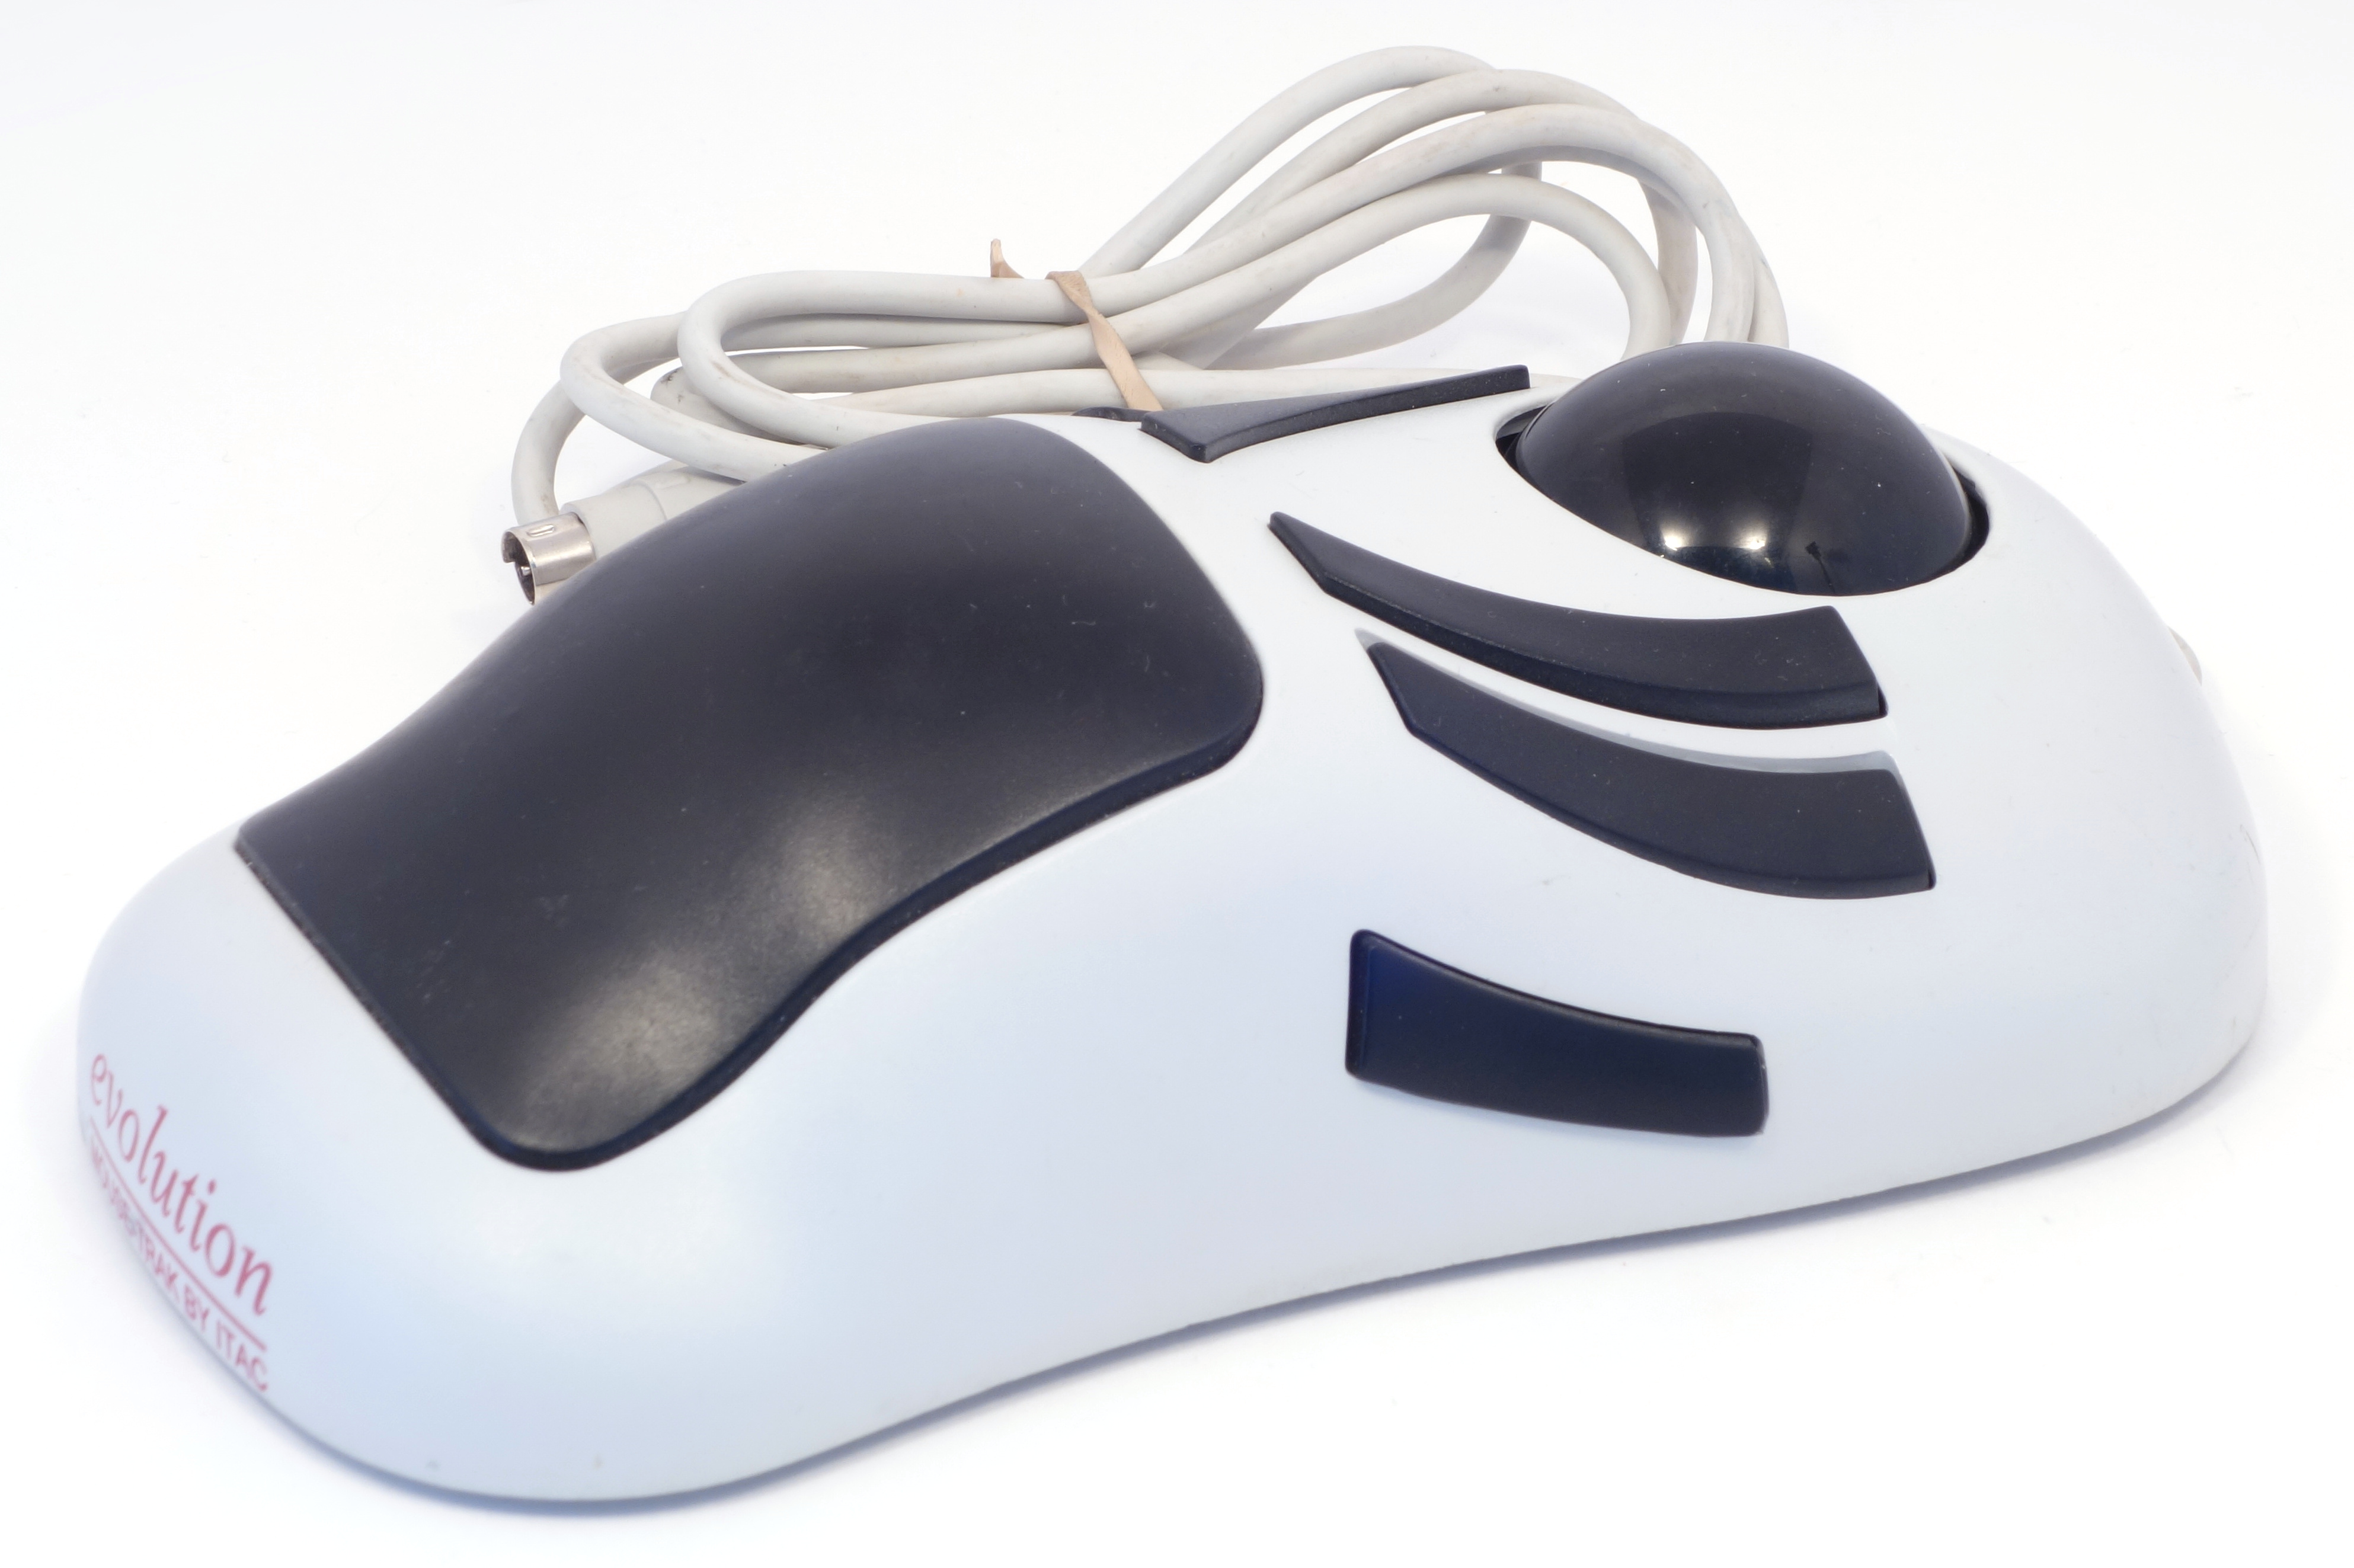
\includegraphics[scale=0.3]{1997_mousetrak_evolution/pic_30.jpg}
    \caption{The evolution MOUSE-TRAK trackball}
    \label{fig:evolutionMOUSE-TRAK}
\end{figure}

The figure \ref{fig:evolutionMOUSE-TRAKTopBottom} shows the top and bottom sides of the trackball.

\begin{figure}[h]
    \centering
    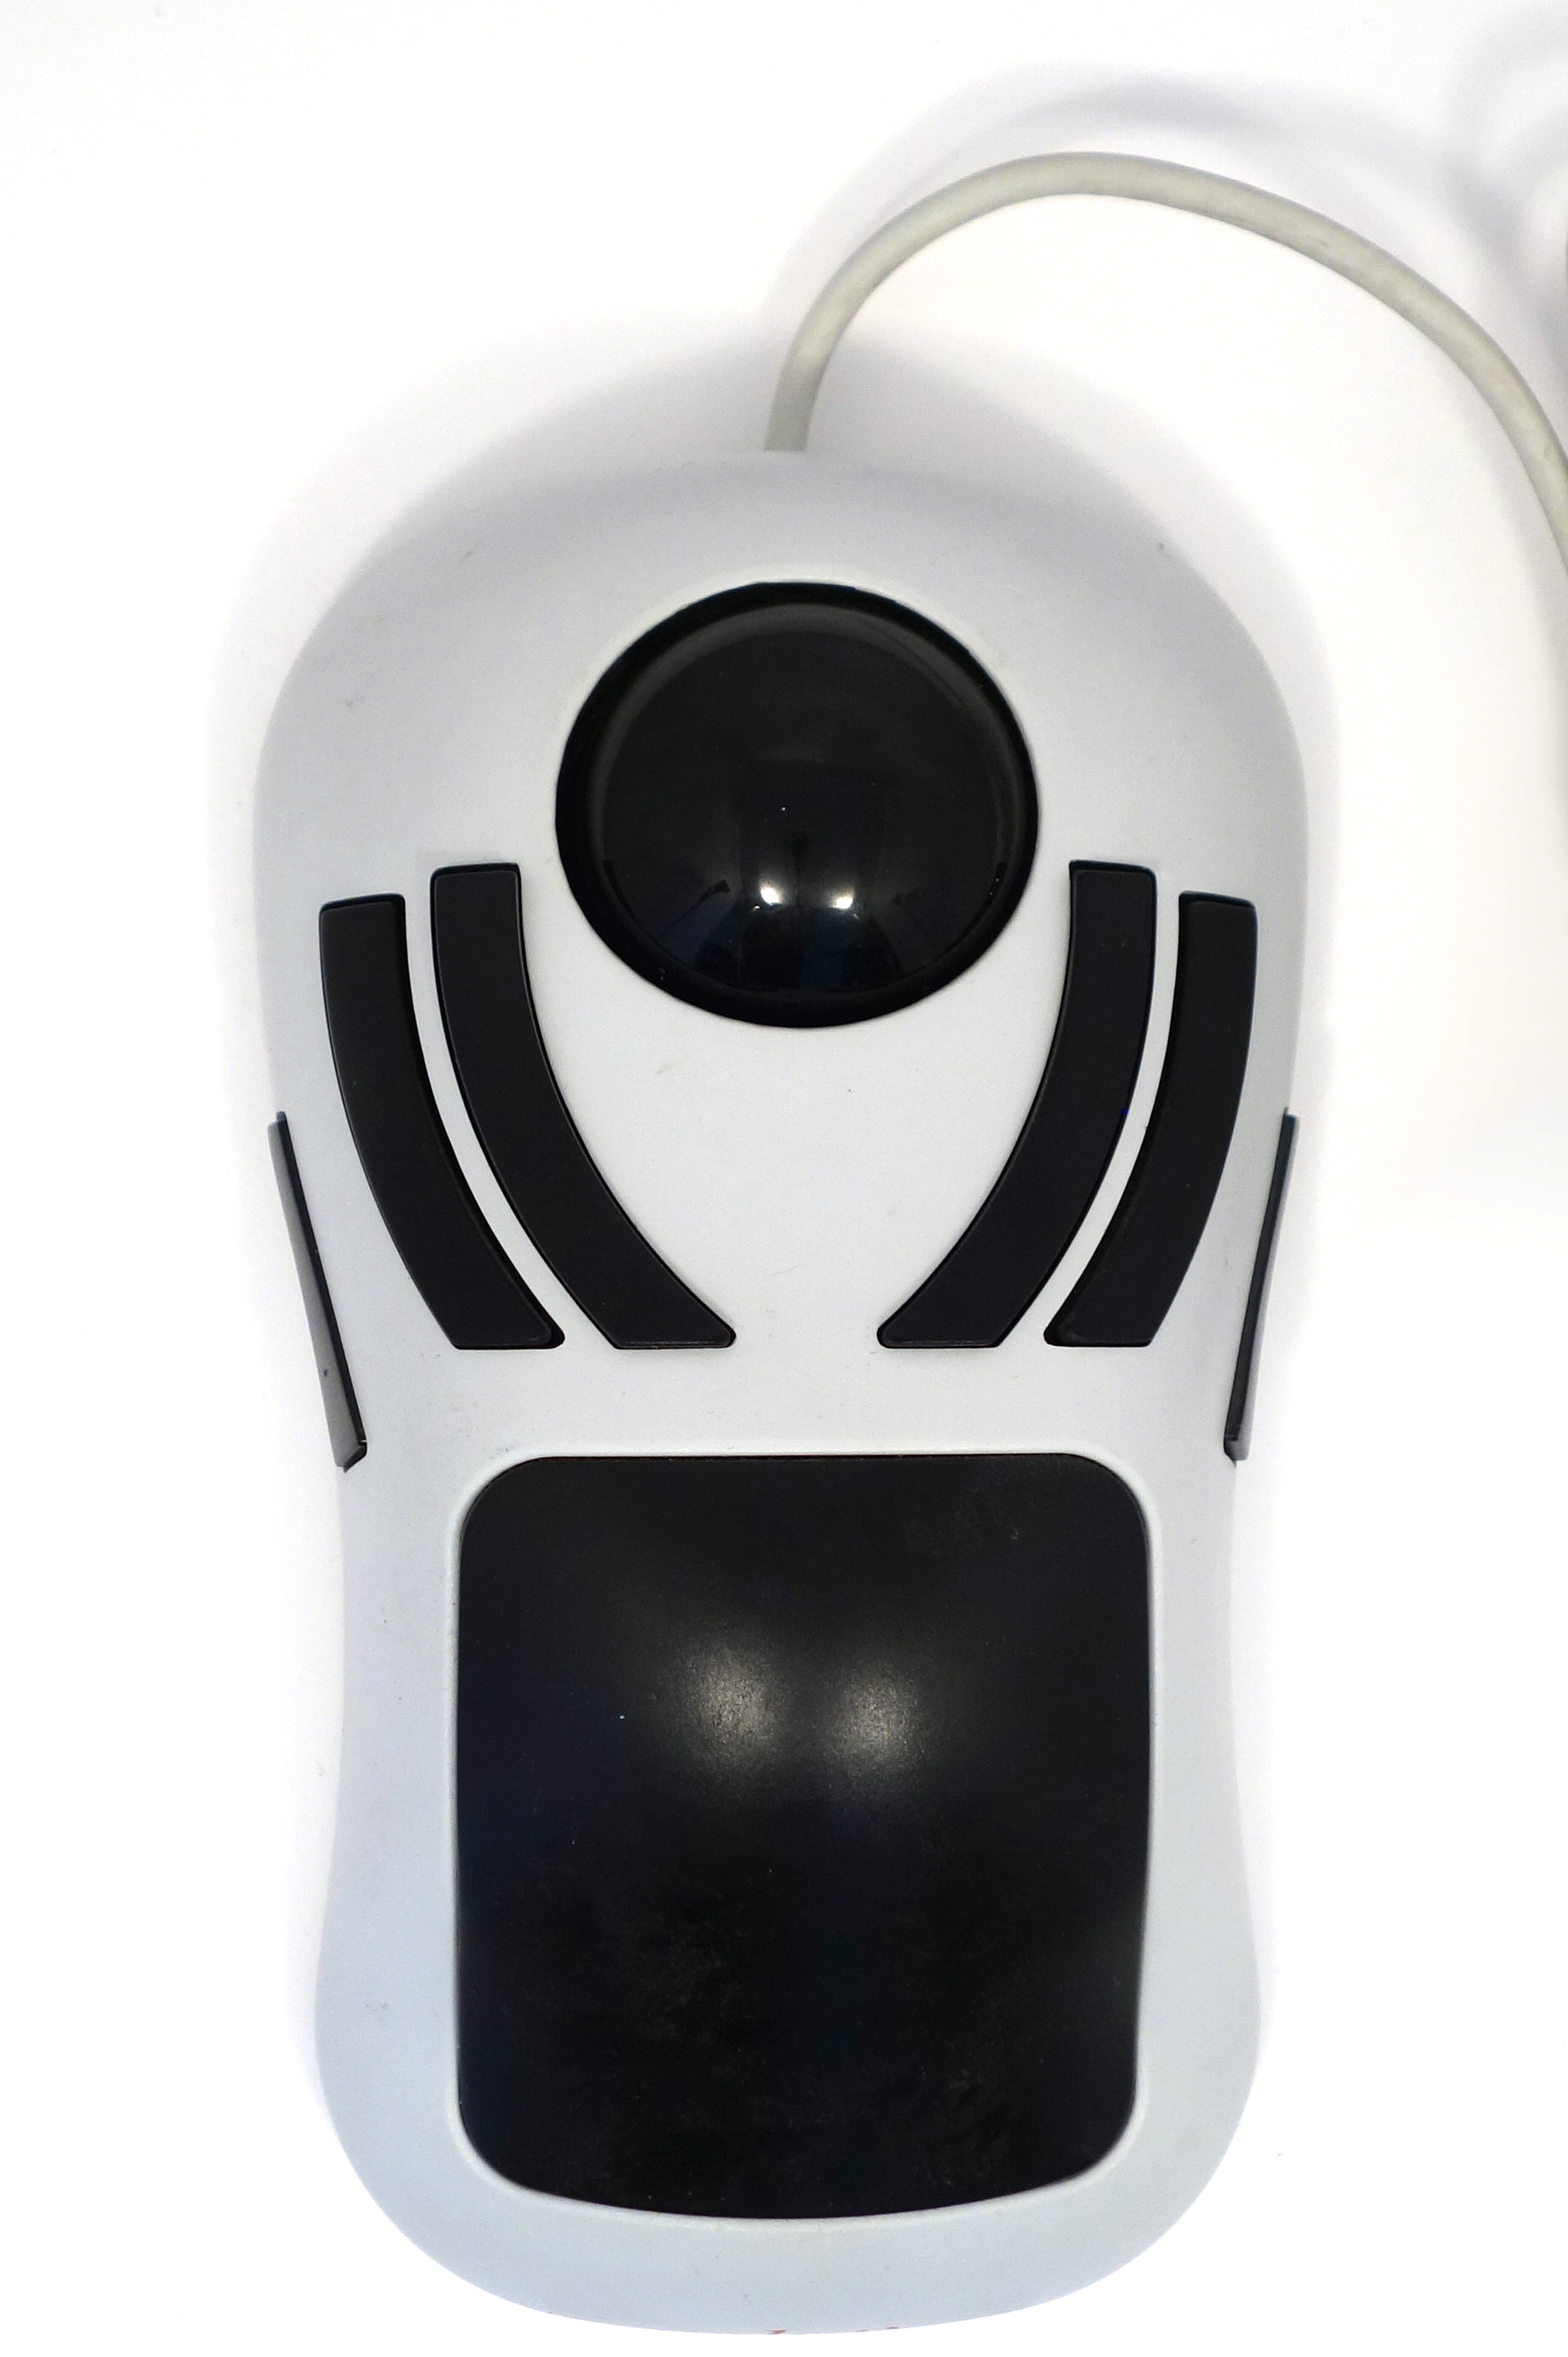
\includegraphics[scale=0.35]{1997_mousetrak_evolution/top_60.jpg}
    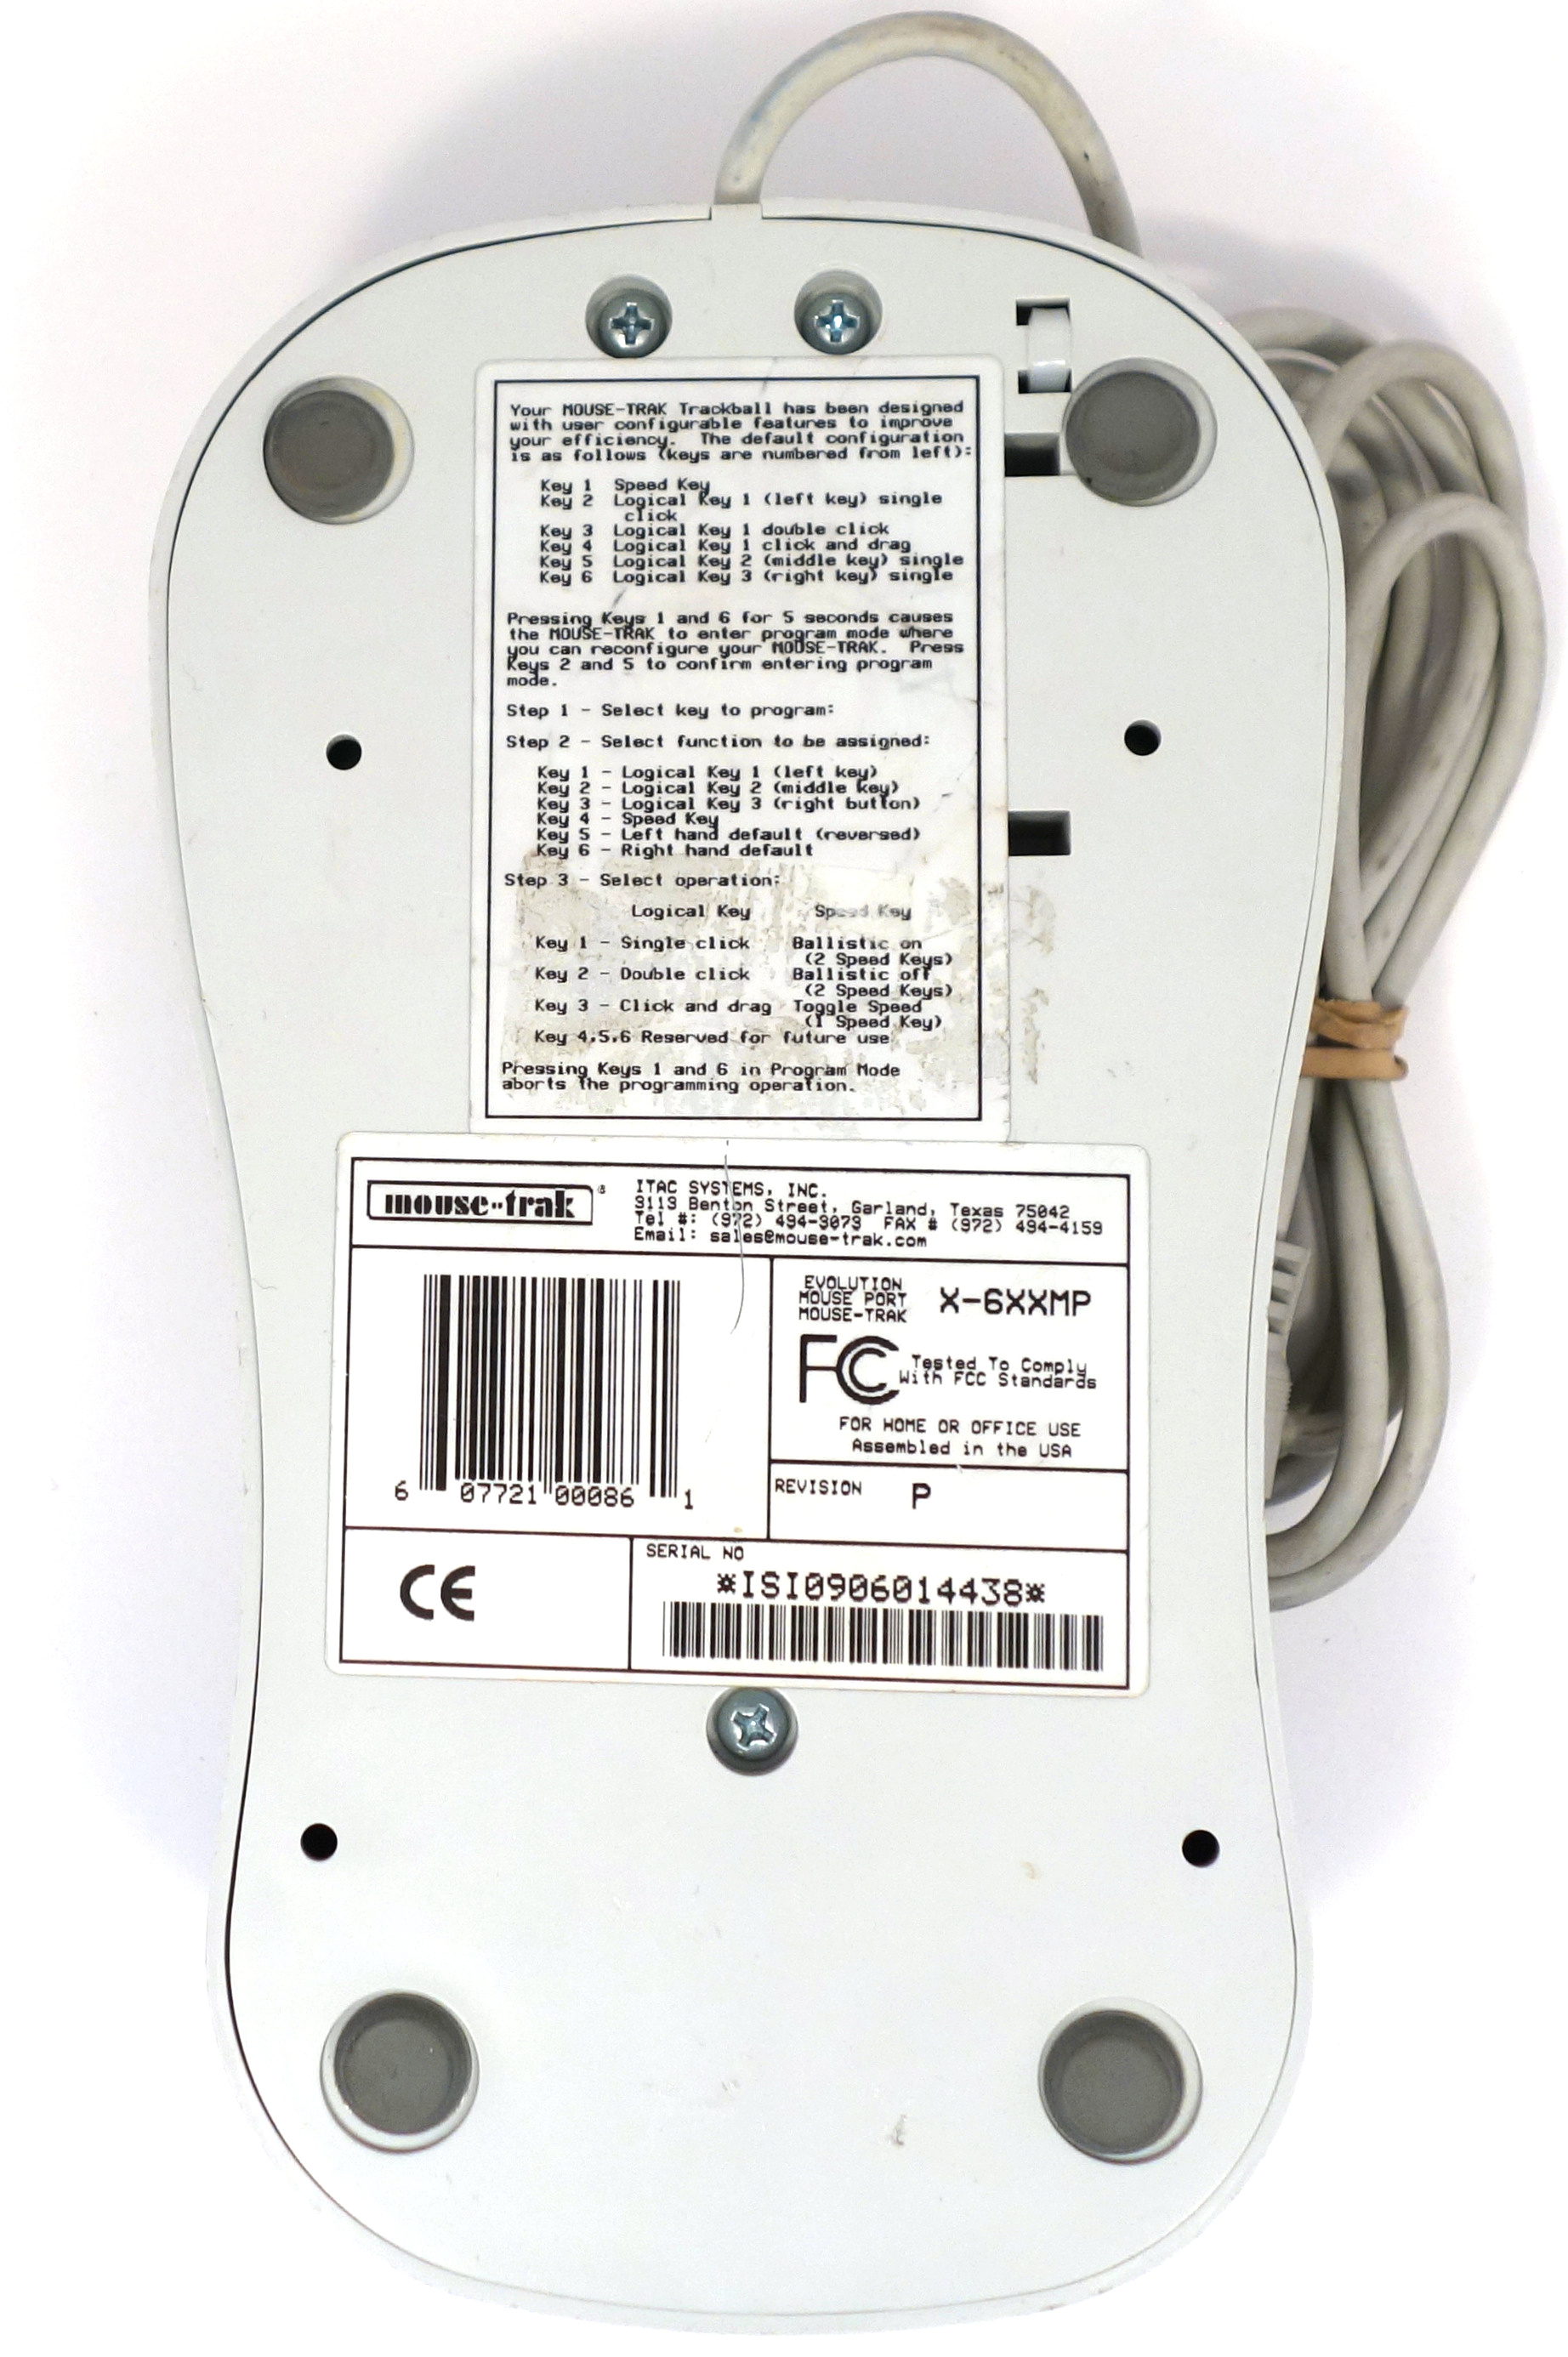
\includegraphics[scale=0.35]{1997_mousetrak_evolution/bottom_60.jpg}
    \caption{evolution MOUSE-TRAK, top and bottom views}
     \label{fig:evolutionMOUSE-TRAKTopBottom}
\end{figure}

The body has a white matte surface with contrasting black elements -- a ball, six narrow long buttons arranged in a zebra style in front of the ball, and a massive soft PVC hand support. On the bottom of the case there are rubber feet for secure fixation on the table surface, a manufacturer's label and detailed instructions on how to program the trackball buttons.

This device is quite large (fig. \ref{fig:evolutionMOUSE-TRAKSize}). Due to the highly elevated arm support, designed to reduce the risk of RSI syndrome, the ball is recessed into the body and visually appears smaller than it actually is.

\begin{figure}[h]
    \centering
    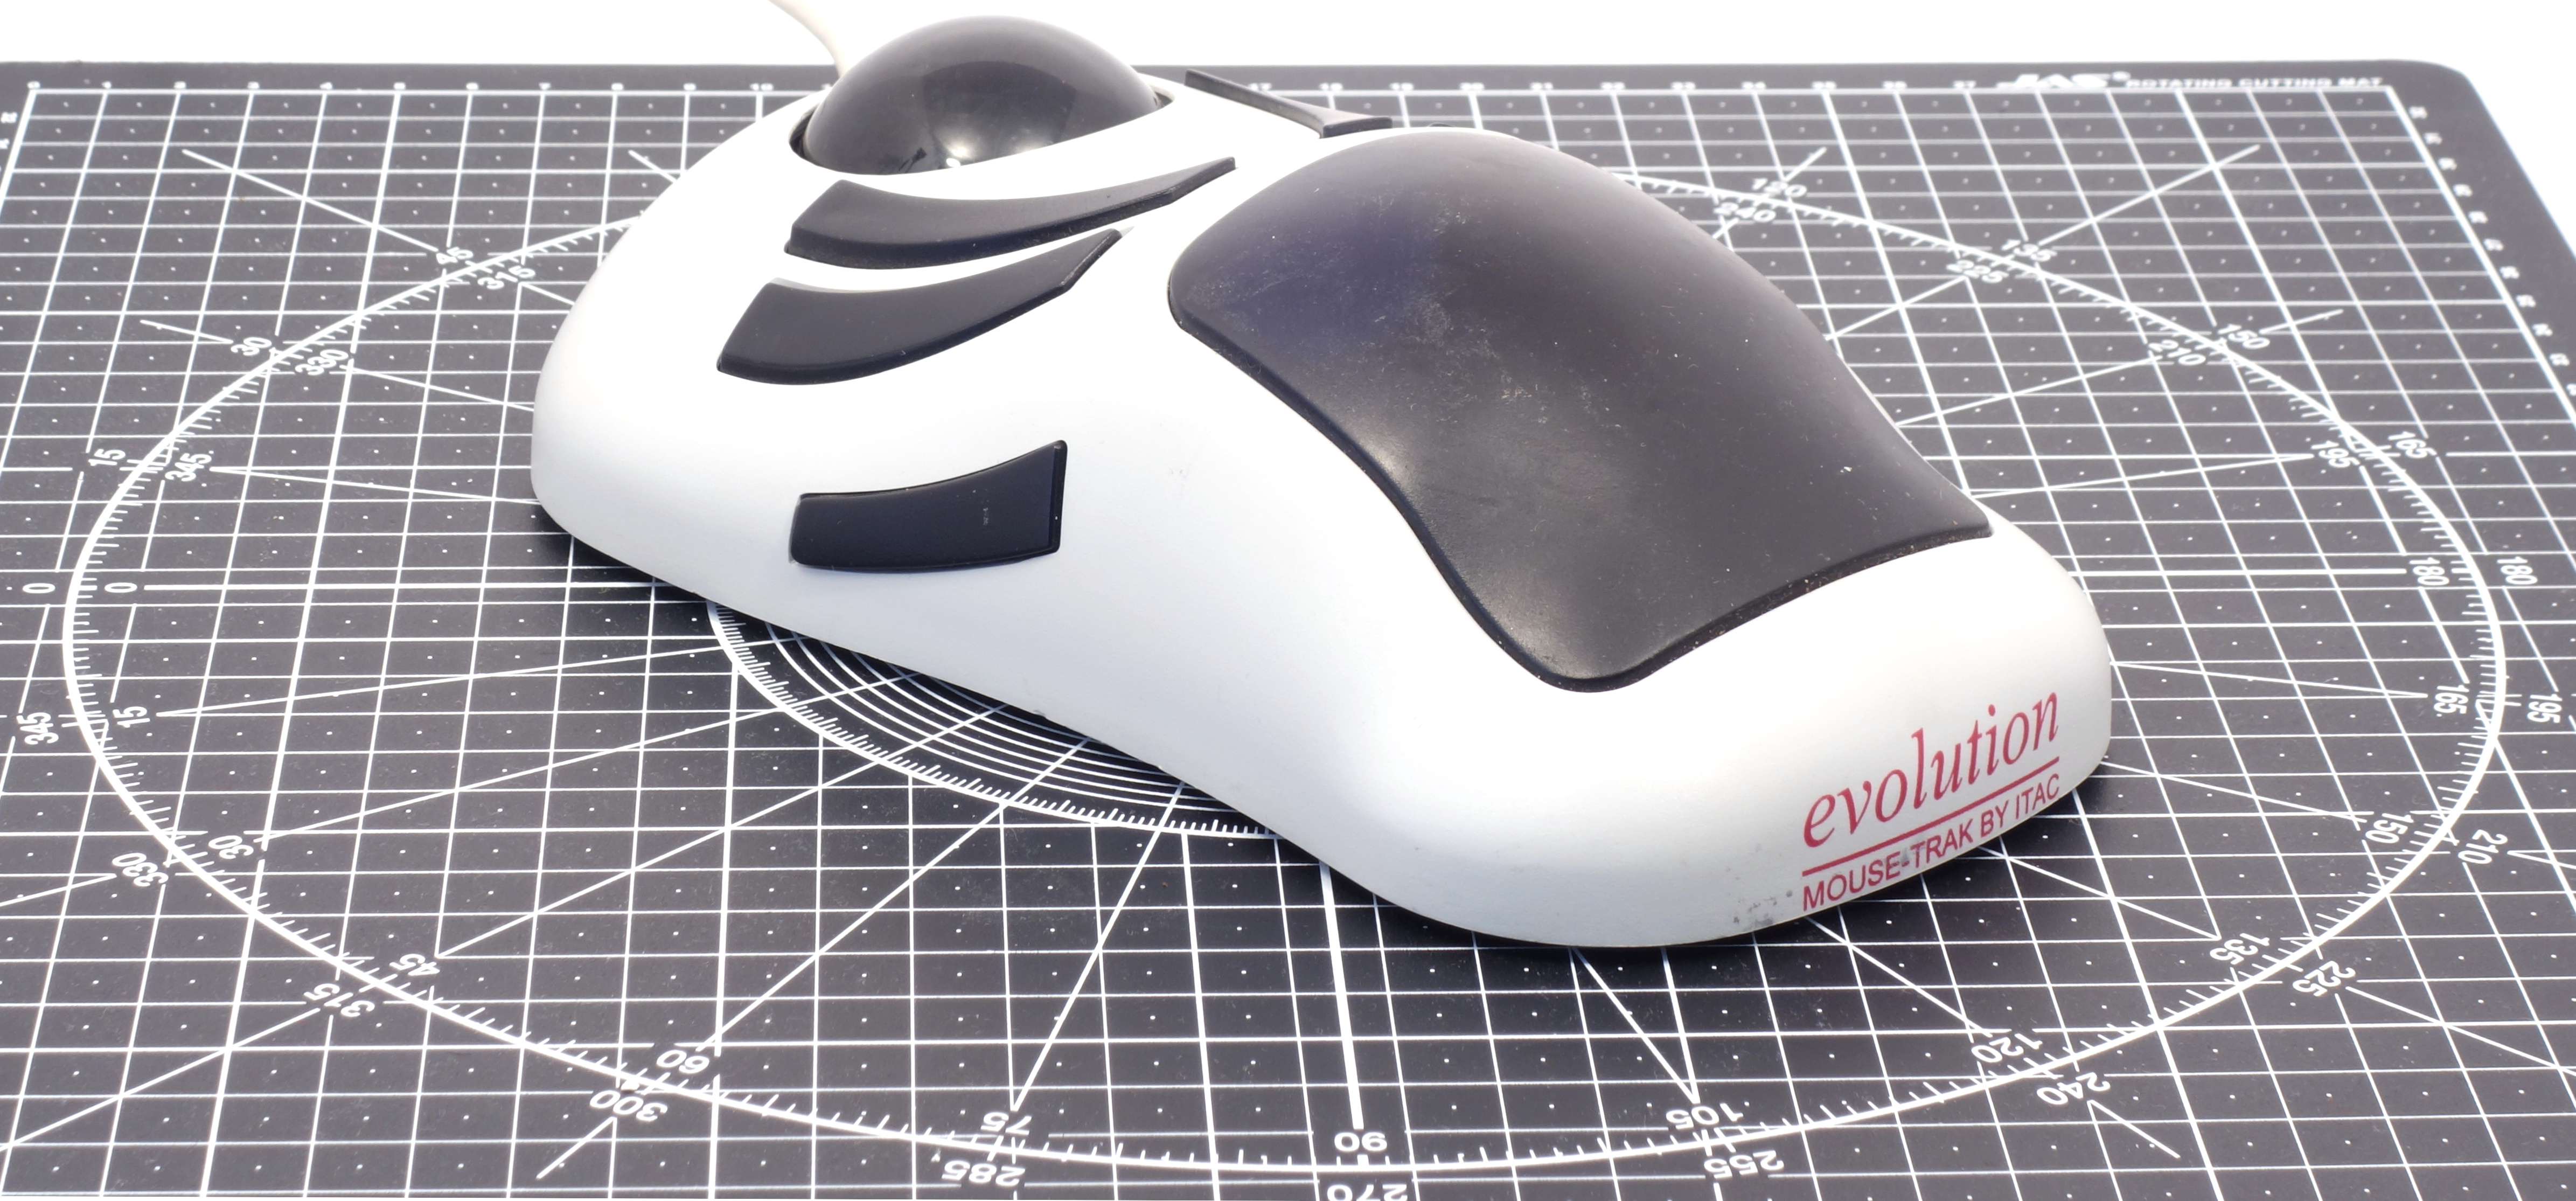
\includegraphics[scale=0.35]{1997_mousetrak_evolution/size_30.jpg}
    \caption{evolution MOUSE-TRAK on a graduated pad with a grid step of 1~cm}
    \label{fig:evolutionMOUSE-TRAKSize}
\end{figure}

The trackball is symmetrical and equally comfortable when used with both right and left hands (especially considering the driver-free button remapping).
The buttons are designed to be pressed with the thumb and little finger \cite{pcmag}, while the rest of the fingers are left to position the cursor (fig. \ref{fig:evolutionMOUSE-TRAKHand}). At the same time, as conceived by the developers, the assignment of the most frequently used functions to the keys located near the ball makes it convenient to use the trackball for users with a smaller hand size.

The reconfiguration mode is turned on by successively pressing a pair of button combinations, after which, also by successive pressing, their functions are reassigned (as already mentioned, detailed instructions are located at the bottom side).

The default buttons configuration is as follows (from left to right): speed adjustment, single left mouse button click, double left mouse button click, left mouse button click with hold (used for dragging), single middle mouse button click, and single right mouse button click \cite{advanced}.

The trackball was produced in two versions with different interfaces (PS/2 and USB).

\begin{figure}[h]
    \centering
    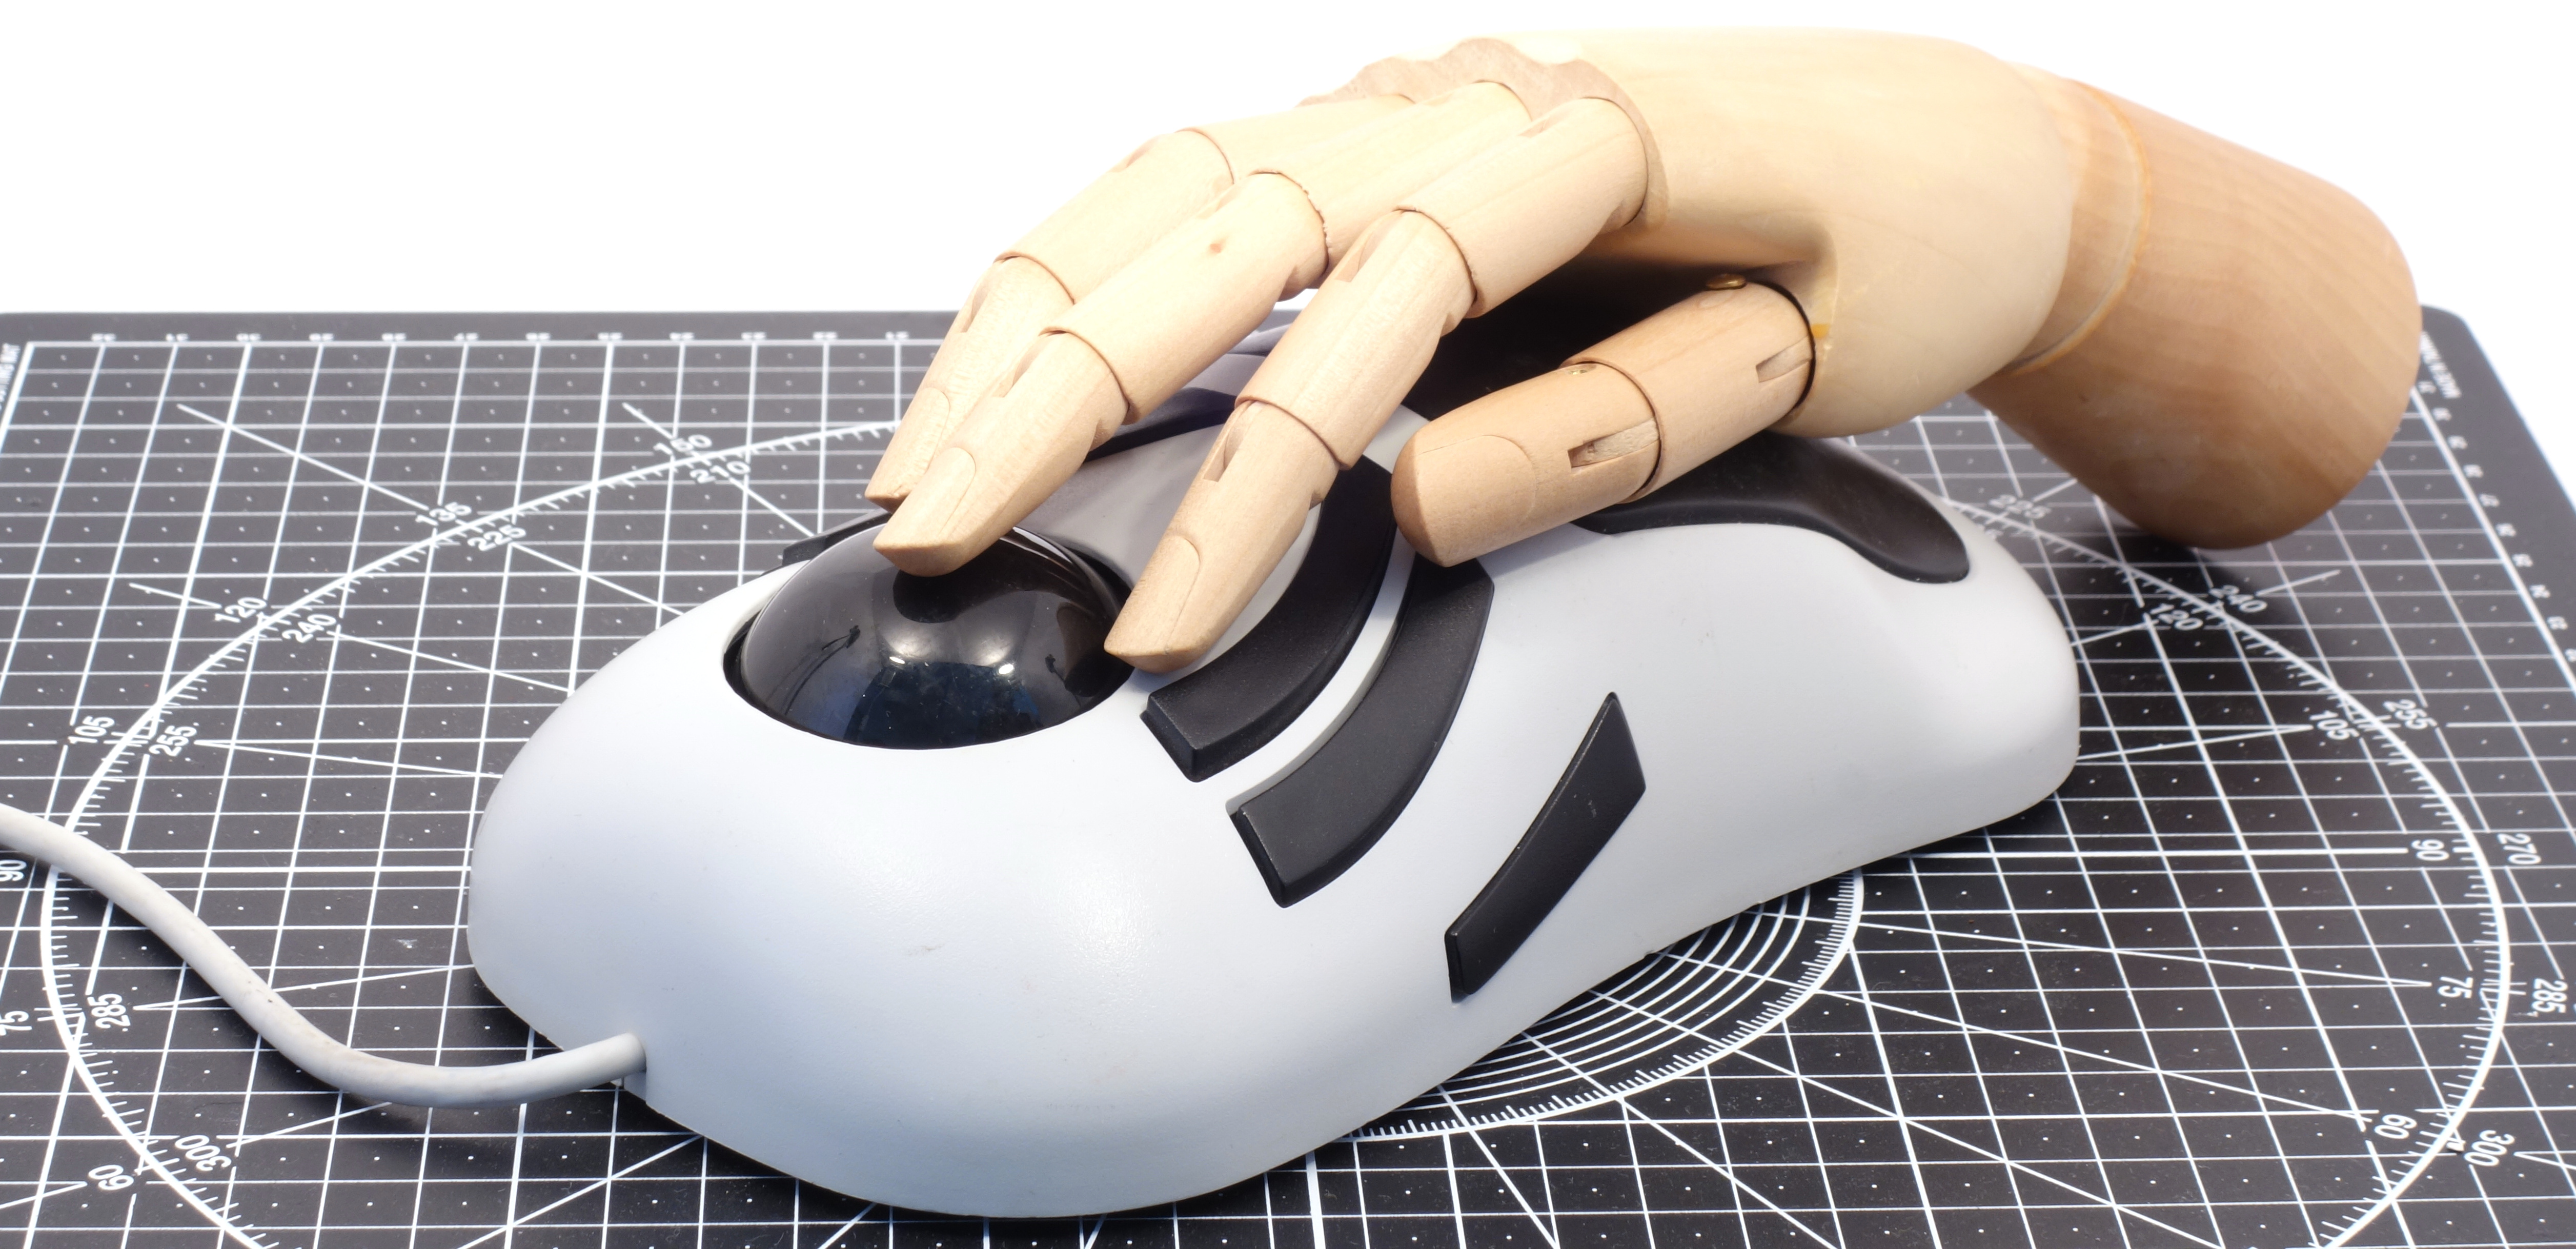
\includegraphics[scale=0.35]{1997_mousetrak_evolution/hand_30.jpg}
    \caption{evolution MOUSE-TRAK with a human hand model}
    \label{fig:evolutionMOUSE-TRAKHand}
\end{figure}

The trackball internals are shown in fig. \ref{fig:evolutionMOUSE-TRAKInside}. As you can see, it uses a classic optomechanical scheme. The rollers are made with ball bearings and metal shafts, which ensures maximum reliability and durability of the structure. This is also noted in the manufacturer's description, which emphasizes the use of bearings and rollers made of hardened steel among the features of the device.

The disadvantages of the design include the lack of a removable latch ring: given that the ball is recessed inside the case, it is impossible to remove it for cleaning without disassembling the trackball.

\begin{figure}[h]
    \centering
    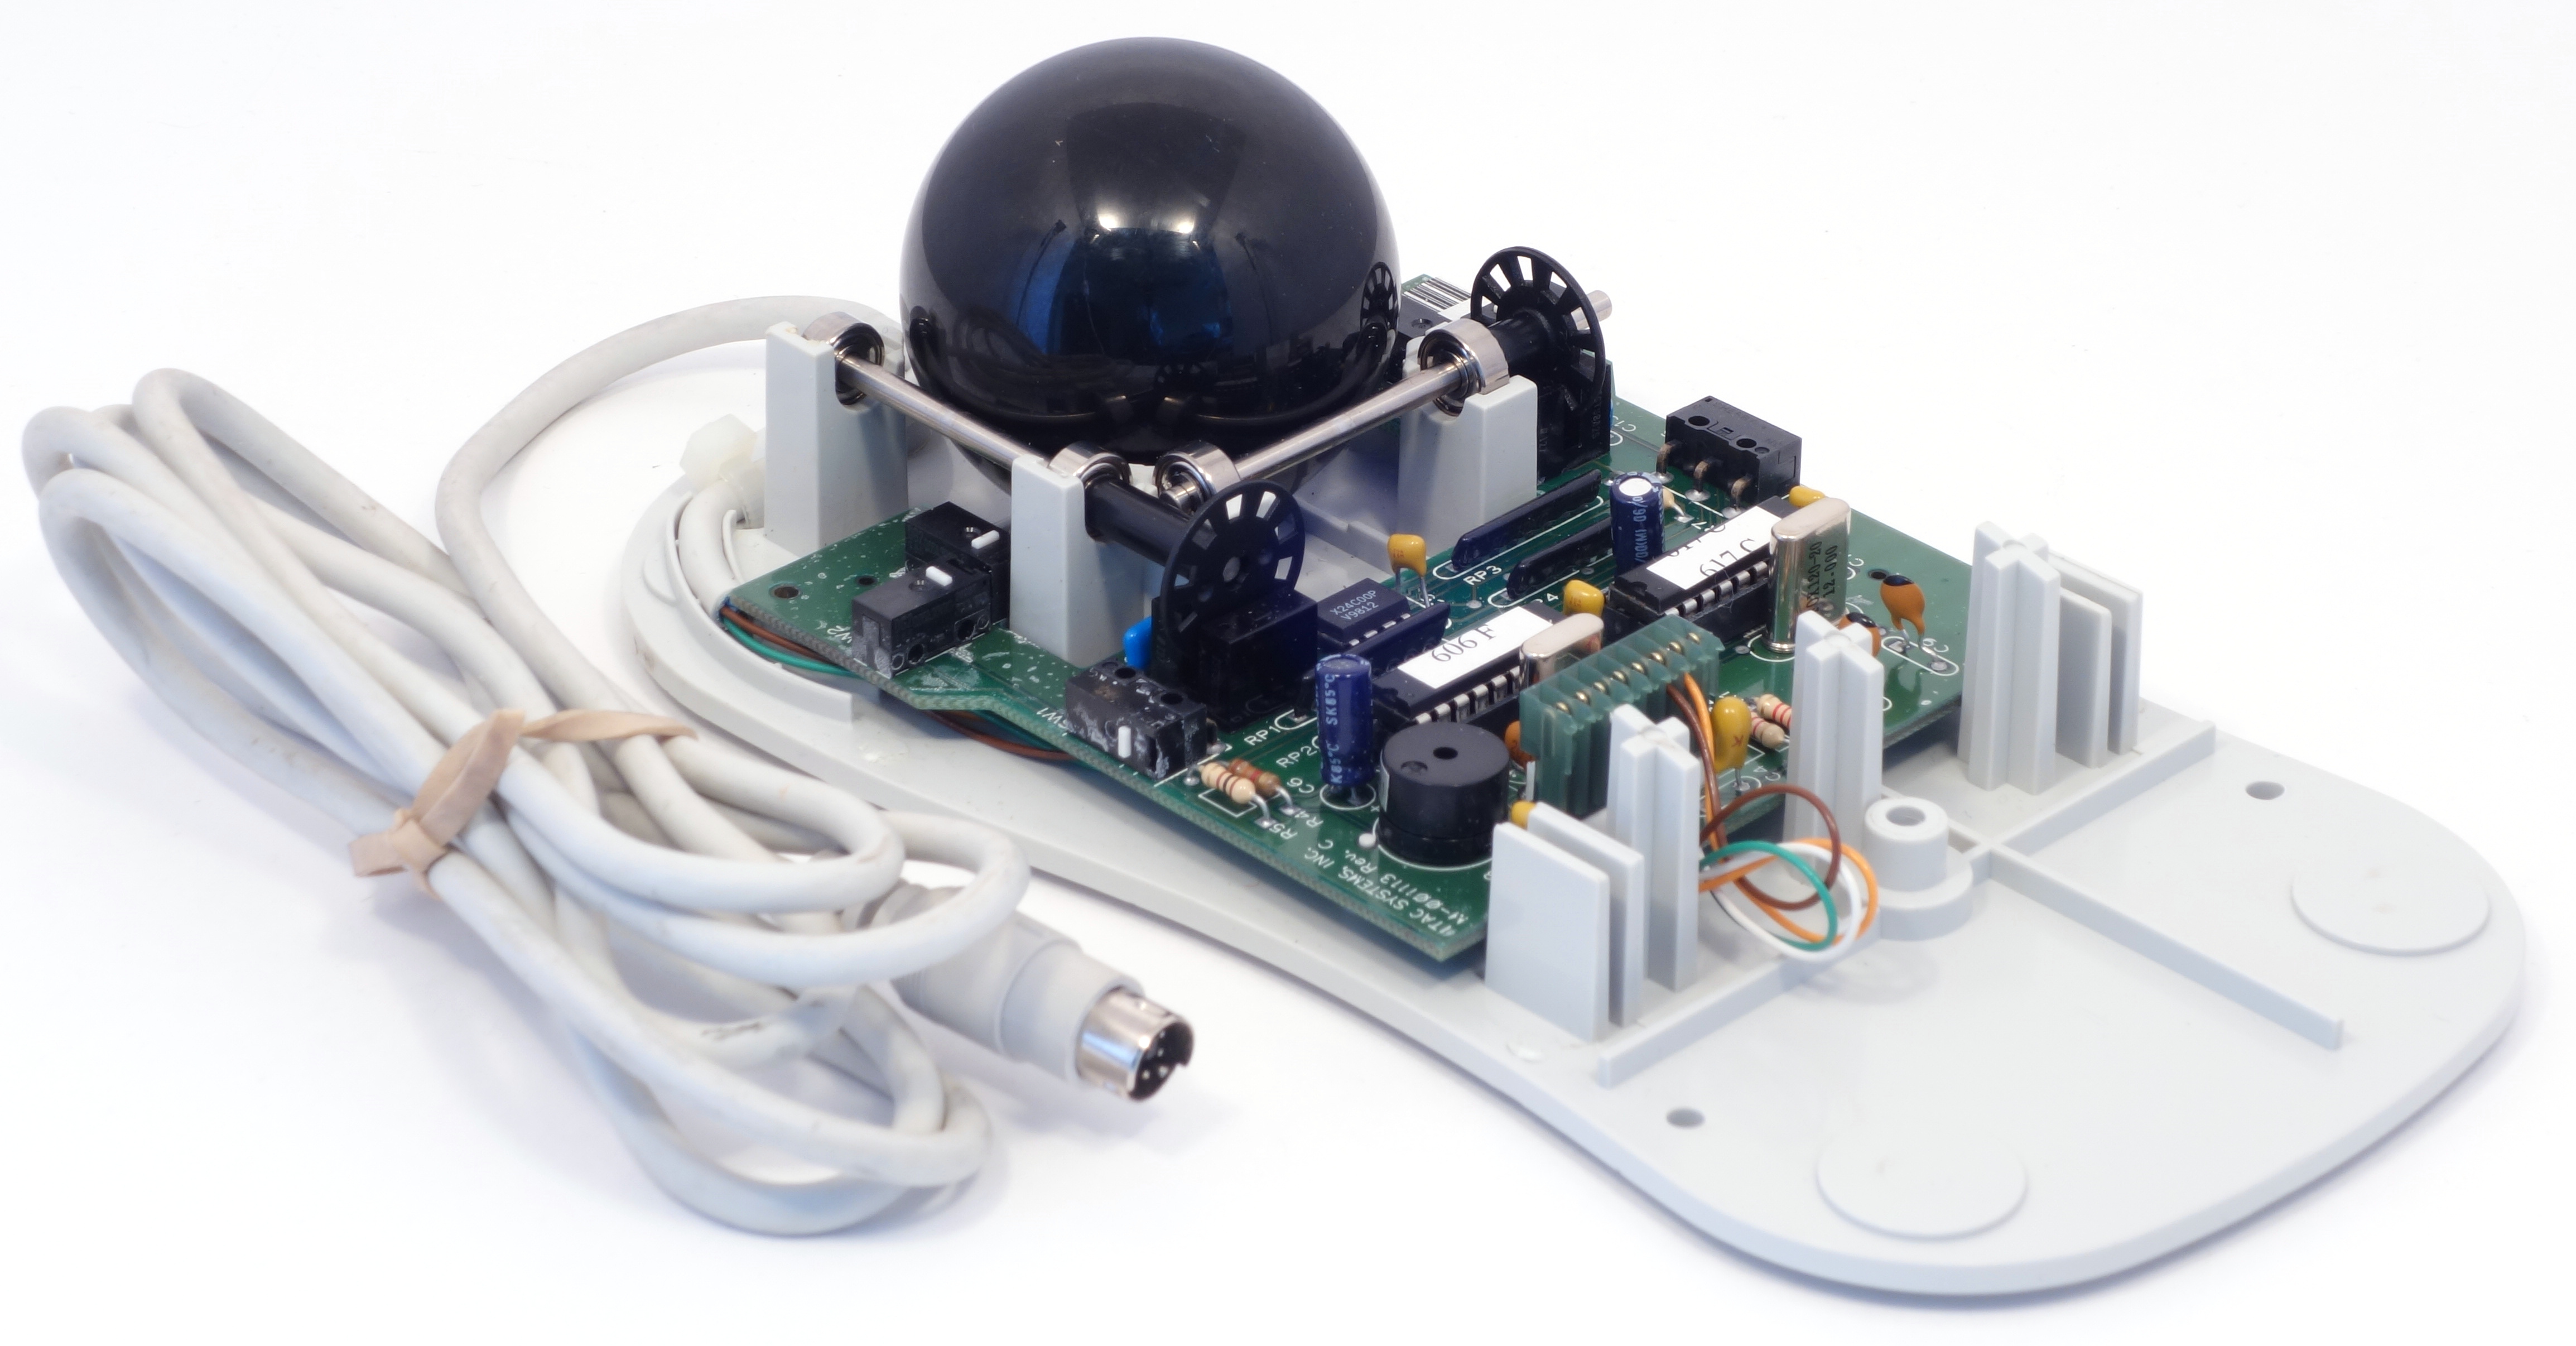
\includegraphics[scale=0.5]{1997_mousetrak_evolution/inside_30.jpg}
    \caption{evolution MOUSE-TRAK disassembled}
    \label{fig:evolutionMOUSE-TRAKInside}
\end{figure}

\begin{thebibliography}{9}
\bibitem{announcement} ITAC Systems announces evolution MOUSE-TRAK \url{https://web.archive.org/web/19970116093947/http://www.mousetrak.com/evol.htm}
\bibitem{description} evolution MOUSE-TRAK BY ITAC \url{https://web.archive.org/web/19980116135700/http://mousetrak.com:80/index.html}
\bibitem{pcmag} M.N. Rusignuolo. Playing Cat -- and Mouse // PC MAGAZINE, October 7, 1997. -- p. 37 \url{https://books.google.by/books?id=oOfsp5YznnkC&lpg=PA37&dq=evolution%20mouse-trak&pg=PA37#v=onepage&q=evolution%20mouse-trak&f=false}
\bibitem{advanced} Evolution advanced programming procedures \url{https://web.archive.org/web/19980116134309fw_/http://mousetrak.com/evol3.htm}
\end{thebibliography}
\end{document}
